\documentclass[a4paper,12pt,spanish]{article}

% Fonts.
\usepackage{mathpazo}
\usepackage[scaled=1.03,varqu]{zi4}
%\usepackage[scaled=0.92]{luximono}
\usepackage[T1]{fontenc}
\usepackage[utf8]{inputenc}
\usepackage{babel}

% Format.
\usepackage{geometry}
\geometry{verbose,tmargin=3cm,bmargin=3cm,lmargin=3cm,rmargin=3cm}
\usepackage{setspace}
\onehalfspacing

% Referències.
\usepackage[unicode=true,
        bookmarks=true,bookmarksnumbered=false,bookmarksopen=false,
        breaklinks=false,pdfborder={0 0 0},backref=false,colorlinks=false]
    {hyperref}
\hypersetup{pdfauthor={Gispert Sánchez, Francesc; Lorente García, Ester; Martín Alaminos, David}}

% Gràfics.
\usepackage{graphicx}
\usepackage{subfig}
\usepackage{standalone}
\usepackage{afterpage}
\usepackage{pdflscape}

% Codi.
\usepackage{listings}
\lstset{
    inputencoding=utf8,
    extendedchars=true,
    aboveskip=20pt,
    belowskip=10pt,
    captionpos=b,
    frame=single,
    basicstyle=\small\ttfamily,
    numbers=left,
    numberstyle=\scriptsize,
    stepnumber=1,
    numbersep=5pt,
    columns=full_flexible,
    showspaces=false,
    showtabs=false,
    breaklines=true,
    literate=%
        {á}{{\'a}}1%
        {é}{{\'e}}1%
        {í}{{\'i}}1%
        {ó}{{\'o}}1%
        {ú}{{\'u}}1%
        {Á}{{\'A}}1%
        {É}{{\'E}}1%
        {Í}{{\'I}}1%
        {Ó}{{\'O}}1%
        {Ú}{{\'U}}1%
        {¿}{{?`}}1%
        {¡}{{!`}}1%
}
\renewcommand{\lstlistingname}{Texto}
\newcommand{\lstlistingautorefname}{\lstlistingname}


\begin{document}

\title{
    {\huge Inteligencia artificial}\\ 
    Planificación
}

\author{
    Gispert Sánchez, Francesc-Xavier\\
    Lorente García, Ester\\
    Martín Alaminos, David
}

\maketitle

\noindent \rule[0.5ex]{1\columnwidth}{1pt}
%\clearpage

\tableofcontents

\clearpage

%%%%%%%%%%%%%%%%%%%%%%%%%%%%%%%%%%%%%%%%%%%%%%%%%%%%%%%%%%%%%%%%%%%%%%%%%%%%%%%%


\section{Introducción y descripción del problema} \label{sec:intro}

Algunos problemas de optimización resultan computacionalmente intratables con 
los algoritmos exactos que se conocen a causa de su complejidad algorítmica, 
debida a la magnitud de la estructura combinatoria subyacente. Por ello, la 
inteligencia artificial utiliza técnicas que podan el espacio de búsqueda y 
lo inspeccionan guiadas por heurísticas para poder ofrecer soluciones 
aproximadas de forma sencilla. 

Una familia de problemas cuya resolución se ha simplificado mucho con 
herramientas genéricas que automatizan este proceso de búsqueda es la de los 
problemas de planificación. El objetivo de estos problemas es construir un 
plan o secuencia de acciones que permitan llegar a un cierto objetivo 
partiendo de un estado inicial. Se trata, pues, de problemas de síntesis, en 
los que hay que construir una solución basándose en el conocimiento del 
dominio (en este caso, en el estado del entorno, las acciones disponibles en 
cada momento y el objetivo al que se desea llegar).

La comunidad de inteligencia artificial ha desarrollado, a lo largo de los 
años, herramientas capaces de resolver problemas de planificación 
independientemente del dominio. Así, el usuario de estas herramientas solo 
tiene que modelizar su dominio y su problema mediante un lenguaje formal de 
representación y el sistema se encarga de la resolución automática del 
problema. 

En este trabajo, lo ejemplificamos mediante la resolución de un problema 
simple de asignación que se puede modelizar como un problema de planificación 
para guiar adecuadamente la construcción de la asignación. El problema 
consiste en la distribución de \(T\) tareas de programación entre \(P\) 
programadores. Cada tarea tiene asociada un nivel de dificultad (\(1\), \(2\) 
o \(3\), por orden creciente) y un tiempo estimado de desarrollo (un número 
de horas); por su lado, cada programador tiene asociada un nivel de habilidad 
(\(1\), \(2\) o \(3\), por orden creciente) y una categoría según su calidad 
(\(1\) o \(2\), por orden decreciente). Un programador puede resolver una 
tarea del mismo nivel de dificultad que su nivel de habilidad en el tiempo 
establecido o bien una tarea con un nivel de dificultad inmediatamente 
superior a su habilidad añadiendo dos horas adicionales. Tras la resolución 
de una tarea, se crea una tarea de revisión de una hora si el programador era 
de primera calidad o de dos horas en caso contrario, independientemente de si 
el programador que la lleva a cabo tiene una habilidad inferior; esta tarea de 
revisión tiene la misma dificultad que la inicial y tiene que ser llevada a 
cabo por otro programador distinto.

En esta práctica hemos considerado la versión básica del problema y las cuatro 
extensiones propuestas, de forma incremental. El problema básico consiste en 
la resolución directa del problema de asignación sin tener en cuenta las 
tareas de revisión. En la primera extensión, se añaden estas tareas de 
revisión al problema. La segunda extensión pretende, además, minimizar el 
tiempo total de resolución de las tareas. En la tercera extensión se limita 
el número de tareas por programador a \(2\) para facilitar el trabajo en 
paralelo. Finalmente, en la cuarta extensión, se pretende minimizar la 
suma del número de personas con tareas asignadas y el tiempo total de 
resolución.

Se desarrolla, pues, un modelo expresado en \texttt{PDDL} para cada uno de los 
problemas considerados, analizando los elementos necesarios y las diferencias 
entre ellos, y se resuelven utilizando la herramienta de planificación 
\texttt{Fast Forward}. El desarrollo de la práctica, así como la estructura 
de este informe, está influenciado por la metodología de la ingeniería del 
conocimiento vista en la práctica anterior, con un desarrollo incremental y 
basada en distintos prototipos (aunque en este caso, debido a la simplicidad 
del problema, las fases de identificación del problema, conceptualización y 
formalización prácticamente se han unido en una sola).

En el resto de este documento, explicamos los pasos del desarrollo de nuestra 
solución y mostramos y analizamos los resultados obtenidos.

\clearpage





\section{Modelización} \label{sec:modelo}

En esta sección se describen detalladamente los elementos que aparecen en los 
modelos desarrollados para cada una de las versiones del problema 
consideradas. Como se explica en la \autoref{sec:implem}, el modelo para cada 
extensión se ha construido añadiendo funcionalidades al modelo para la 
extensión previa. Por lo tanto, y para evitar repeticiones innecesarias, para 
cada extensión solo se detallan los cambios introducidos.


\subsection{Problema básico} \label{sec:mod-basico}

%%% TODO





\subsection{Primera extensión} \label{sec:mod-ext1}

%%% TODO





\subsection{Segunda extensión} \label{sec:mod-ext2}

En esta extensión, se empieza a tener en cuenta el tiempo de realización de 
las tareas. Esto significa que hay que modificar las acciones adecuadamente 
para poder contabilizarlo y tener en cuenta las diferentes circunstancias que 
incrementan el tiempo de realización o de revisión (explicadas en la 
\autoref{sec:intro}).

Añadimos, pues, una nueva función llamada \texttt{(ttotal)} utilizada para 
almacenar el tiempo total de realización de tareas (incluyendo las de 
revisión) de la asignación parcial calculada hasta el momento. Esta función 
se utiliza como valor a minimizar en esta extensión. Además, su valor deberá 
ser actualizado con cada acción de asignación de tareas.

Por otro lado, en esta extensión no basta con saber que hay que realizar una 
tarea de revisión, sino que se necesita saber también cuánto tiempo requiere 
esta. El tiempo de revisión de una tarea depende de la calidad del programador 
que la haya desempeñado previamente. Por lo tanto, una posibilidad sería 
ampliar la acción \texttt{revisa} para que usase como parámetro el programador 
al cual se había asignado la tarea y calcular el tiempo de revisión según la 
calidad de este. Sin embargo, en este caso se ha optado por la introducción de 
dos nuevos predicados, \texttt{(por\_revisar\_1 ?t - tarea)} y 
\texttt{(por\_revisar\_2 ?t - tarea)} que indican que una tarea \texttt{?t} 
comporta una tarea de revisión de una hora o de dos, respectivamente. 

En particular, el efecto de la acción \texttt{realiza} debe adaptarse a estos 
cambios. Concretamente, cuando se ejecuta \texttt{realiza} con una tarea 
\texttt{?t} y un programador \texttt{?p}, se incrementa \texttt{ttotal} con 
el tiempo de realización de \texttt{?t} (incluyendo las dos horas adicionales 
por la habilidad de \texttt{?p} si cabe) y se activa uno de los dos predicados 
\texttt{por\_revisar\_1} o \texttt{por\_revisar\_2} según la calidad de 
\texttt{?p}.

La acción \texttt{revisa} también se adapta del mismo modo. Por un lado, 
cuando se unifica esta acción con una tarea \texttt{?t} y un programador 
\texttt{?p}, en la precondición se comprueba que uno de los dos predicados 
\texttt{(por\_revisar\_1 ?t)} o bien \texttt{(por\_revisar\_2 ?t)} se cumpla 
en vez de comprobar \texttt{(servida ?t)}; por otro lado, en el efecto se 
añade un incremento de \texttt{ttotal} en una o dos horas según el caso.







\subsection{Tercera extensión} \label{sec:mod-ext3}

%%% TODO





\subsection{Cuarta extensión} \label{sec:mod-ext4}

%%% TODO






\subsection{Instancias del problema} \label{sec:mod-inst}

Hasta el momento se ha explicado como se modeliza el dominio de cada versión 
del problema. Del mismo modo, también hay que formalizar utilizando 
\texttt{PDDL} las entradas de los problemas a resolver.

Como se ha explicado, los únicos objetos del problema son las tareas y los 
programadores (cada uno con su propio tipo para reducir el número de posibles 
unificaciones). La entrada de un problema consiste, pues, en una enumeración 
de las tareas y de los programadores considerados seguida de una descripción 
de sus características. Es decir, se inicializan las funciones que 
corresponden a la dificultad y el tiempo necesario para cada tarea y a la 
habilidad y la calidad de cada programador. Esta parte de la descripción es 
común para todas las versiones del problema expuestas.

Además, algunas de las extensiones requieren de la inicialización de otras 
funciones que se utilizan para mantener guardados valores necesarios para 
construir la solución de forma adecuada. En particular, a partir de la segunda 
extensión hay que inicializar a cero el número de horas de realización de las 
tareas asignadas, a partir de la tercera extensión hay que inicializar el 
número de tareas asignadas a cada programador a cero y en la cuarta extensión 
hay que inicializar el número de programadores que trabajan en las tareas 
asignadas a cero, puesto que en la solución inicial no hay ninguna asignación. 

El estado inicial de la planificación, pues, es una asignación vacía. Esta 
asignación se va completando a medida que el planificador asigna tareas (tanto 
las tareas iniciales como las de revisión) a los programadores. Por lo tanto, 
una solución final se consigue cuando todas las tareas han sido asignadas a 
algún programador. Esto se modeliza en la versión básica del problema (en la 
cual no se consideran las tareas de revisión) pidiendo que todas las tareas 
estén servidas y en todas las extensiones posteriores pidiendo que todas las 
tareas estén revisadas (puesto que, por la definición de las acciones, una 
tarea solo puede estar revisada cuando también está servida). 

Finalmente, en algunas de las extensiones se pide que el planificador intente 
minimizar algunos criterios. Concretamente, en la segunda y en la tercera 
extensiones se intenta minimizar \texttt{(ttotal)} (que representa la suma de 
los tiempos de realización de todas las tareas, incluyendo las de revisión), 
mientras que en la cuarta extensión se intenta minimizar la suma de 
\texttt{(ttotal)} y \texttt{(ntrabajadores)} (que representa el número de 
programadores usados para realizar todas las tareas). 






\clearpage




\section{Implementación} \label{sec:implem}

En la \autoref{sec:modelo}, se ha descrito de forma detallada el modelo 
desarrollado para cada una de las variaciones del problema tratadas; estos 
modelos se encuentran implementados (expresados en el lenguaje \texttt{PDDL}) 
en el código adjunto a este documento. En esta sección, pues, se comenta el 
proceso seguido para su implementación. 

Para implementar el modelo final, se ha optado por un esquema de diseño 
incremental basado en prototipos, siguiendo el guión propuesto en el enunciado 
de la práctica. Es decir, se empezó con una solución para el problema básico 
propuesto, que sirvió esencialmente como toma de contacto con el lenguaje 
\texttt{PDDL} y la herramienta \texttt{Fast Forward}, y esta se fue ampliando 
poco a poco y de forma ordenada para tener en cuenta cada una de las 
extensiones trabajadas. Por lo tanto, a lo largo del desarrollo de la práctica 
se han ido construyendo prototipos, todos ellos perfectamente funcionales, 
cada vez teniendo en cuenta más elementos del problema hasta llegar a la 
última extensión. 

Sin embargo, la implementación del prototipo correspondiente a cada extensión 
partiendo de la anterior se ha llevado a cabo prácticamente en un solo paso 
(o sea, sin desarrollar diversos prototipos intermedios entre una extensión y 
la siguiente), puesto que la estructura en extensiones propuesta en el 
enunciado era suficientemente sencilla (es decir, los añadidos de una 
extensión respecto a la previa eran tan pocos que no justificaba una 
metodología más compleja).

Aparte de los modelos en \texttt{PDDL}, también se ha desarrollado un pequeño 
\textit{script} en \texttt{Python} (se encuentra también en el código adjunto 
a este documento) para la generación aleatoria de instancias de entrada de 
nuestro problema y se ha utilizado para los experimentos descritos en la 
\autoref{sec:res-extra}. 


\clearpage




\section{Resultados} \label{sec:resultados}

%%% TODO


\subsection{Problema básico} \label{sec:res-basico}

En este problema solo se espera que se genere una asignación válida sin tener 
en cuenta el tiempo de ejecución de las tareas ni las tareas de revisión. Por 
lo tanto, las posibilidades a explorar en los juegos de prueba son muy 
limitadas. 

El primer juego de pruebas consiste en tres tareas, una de cada nivel de 
dificultad posible, y dos programadores con niveles de habilidad 1 y 2, 
respectivamente. En este caso, la única restricción es que la tarea de 
dificultad 3 tiene que asignarse al programador de habilidad 2. En este caso, 
el planificador encuentra una solución inmediatamente y sin dificultades.

En el segundo juego de pruebas, en cambio, se elimina el programador con 
nivel de habilidad 2, de manera que es imposible encontrar una asignación que 
satisfaga las restricciones del problema. El planificador es capaz de detectar 
esta situación e informa de la inexistencia de solución correctamente.








\subsection{Primera extensión} \label{sec:res-ext1}

En la primera extensión se añaden las tareas de revisión pero, aun así, las 
posibles pruebas a realizar siguen siendo limitadas. Como en la versión 
básica, pues, se contrasta la respuesta del planificador ante entradas muy 
parecidas pero con ligeras diferencias que hacen que una de ellas sea 
irresoluble.

Así, el primer juego de pruebas consiste en tres tareas de dificultad máxima 
y dos programadores con niveles de habilidad mínima y media. Con esta 
configuración, sería posible asignar todas las tareas al programador de mayor 
habilidad; sin embargo, el hecho de que el encargado de las tareas de revisión 
tenga que ser distinto del programador encargado de las tareas iniciales 
imposibilita construir una solución válida. En conclusión, no existe una 
solución para esta primera entrada y el planificador es capaz de detectarlo.

Por el contrario, en el segundo juego de pruebas los dos programadores pueden
realizar y revisar todas las tareas, pero su calidad es distinta. 
Como esta extensión solo intenta asignar una tarea a un programador sin tener
en cuenta el tiempo, el planificador asigna la realización de las tareas al
programador de calidad 2 y no al de calidad 1.







\subsection{Segunda extensión} \label{sec:res-ext2}

En esta segunda extensión ya se impone un criterio de optimización. Esto 
permite explorar diversos casos construídos expresamente para estudiar si 
el planificador es capaz de encontrar el óptimo o, en caso contrario, cuán 
lejos se encuentra. 

Como no hay ninguna limitación en el número de tareas asignadas a cada 
programador, es fácil darse cuenta de que el óptimo de todos los problemas se 
obtiene cuando las tareas se asignan a los programadores con nivel de 
habilidad mayor o igual que las tareas, si los hay, y de entre estos a los 
programadores de primera calidad cuando sea posible (puesto que el incremento 
del tiempo debido a la habilidad del programador es de dos horas, mientras 
que el incremento del tiempo de revisión debido a la calidad del programador 
es solo de una hora). Esta observación nos permite calcular el óptimo 
``a mano'' en los casos de prueba propuestos y compararlo con la solución 
ofrecida por el planificador.



%%% TODO





\subsection{Tercera extensión} \label{sec:res-ext3}

En esta versión del problema se limita a dos la cantidad de tareas que un 
programador puede tener a su cargo. Se trata, por lo tanto, de una versión 
mucho más restrictiva del problema que requiere más programadores (por lo 
menos, tantos como tareas). 

En el primer juego de pruebas, se consideran cuatro tareas y cuatro 
programadores. Concretamente, hay una tarea de cada nivel de dificultad 
excepto del nivel máximo, que hay dos. En cuanto a los programadores, hay 
dos programadores de primera calidad, uno con nivel de habilidad 3 y otro 
con nivel de habilidad 1, y dos programadores de segunda calidad, con niveles 
de habilidad 1 y 2. Por lo tanto, la solución óptima se obtiene cuando se 
asignan las dos tareas de máxima dificultad al programador de mayor 
habilidad, sus revisiones al único otro programador con habilidad suficiente,
las otras tareas al programador de habilidad 1 y categoría 1 y las revisiones 
de estas al último programador. Esta es, precisamente, la solución que halla 
el planificador automático.

En el segundo juego de pruebas se aumenta el tamaño y se valora el efecto de 
la limitación del número de tareas a programadores. A tal efecto, construimos 
un juego de pruebas con veinte tareas de dificultad máxima y diez 
programadores de habilidad máxima y diez más de habilidad media. Este juego 
de pruebas lo resolvemos según la segunda extensión y esta tercera extensión 
y comparamos los resultados obtenidos. Con la segunda extensión del problema, 
el planificador encuentra una solución en la que asigna todas las tareas a un 
mismo programador y todas las tareas de revisión a otro programador y que 
conlleva un tiempo total de desarrollo de 143 horas (se trata de una solución 
óptima). La solución obtenida con la tercera extensión del problema, por su 
parte, requiere la colaboración de los 20 programadores y resulta en un 
tiempo total de desarrollo de 163 horas. Esta diferencia se explica en parte 
por las tareas que han tenido que ser realizadas por programadores de calidad 
inferior (sin embargo, la solución hallada no es óptima). 

Concluimos, pues, que la limitación del número de tareas por programador 
aumenta la cantidad de horas necesarias, pero la diferencia no es muy 
significativa si el número de programadores es suficiente porque las
penalizaciones (debidas a la poca habilidad o a la baja calidad de los 
programadores) modeladas tienen poco peso en comparación con la duración de 
las tareas.






\subsection{Cuarta extensión} \label{sec:res-ext4}

%%% TODO






\subsection{Evolución respecto al tamaño de la entrada} \label{sec:res-extra}

Como trabajo adicional, hemos desarrollado algunos \textit{scripts} en 
\texttt{Python} para automatizar la generación de instancias aleatorias de 
las distintas versiones del problema y resolverlas utilizando el planificador 
\texttt{Fast Forward}. Estos \textit{scripts} nos han permitido experimentar 
con entradas de distintos tamaños y estudiar la evolución del comportamiento 
del planificador, tanto en lo que respecta a las soluciones obtenidas como 
al tiempo de ejecución del planificador. Todo el código desarrollado se 
incluye en los archivos adjuntos a este documento.

Para esta parte, se han generado distintas entradas de forma aleatoria 
aumentando progresivamente el número de tareas y el número de programadores 
con unos ciertos incrementos constantes. Para cada una de estas entradas, se 
ha resuelto el problema con el planificador y se ha registrado el tiempo de 
ejecución del planificador para encontrar la solución y el tiempo total de 
desarrollo del proyecto según la asignación de tareas a programadores 
obtenida. 

La \autoref{fig:extra-ext2} muestra los resultados obtenidos para la segunda 
extensión. El color de cada una de las curvas representadas identifica los 
incrementos constantes que se han utilizado para la sucesión de problemas 
generados correspondiente. Es decir, si en la leyenda aparece 
\texttt{inc nt($j$) np($k$)}, significa que la línea de ese color representa 
una sucesión de instancias del problema tales que el número de tareas se 
incrementa en $j$ y el número de programadores se incrementa en $k$ entre 
una instancia y la siguiente.

\afterpage{ % Página horizontal (a parte).
\begin{landscape}

    \begin{figure}[ht]
        \centering
        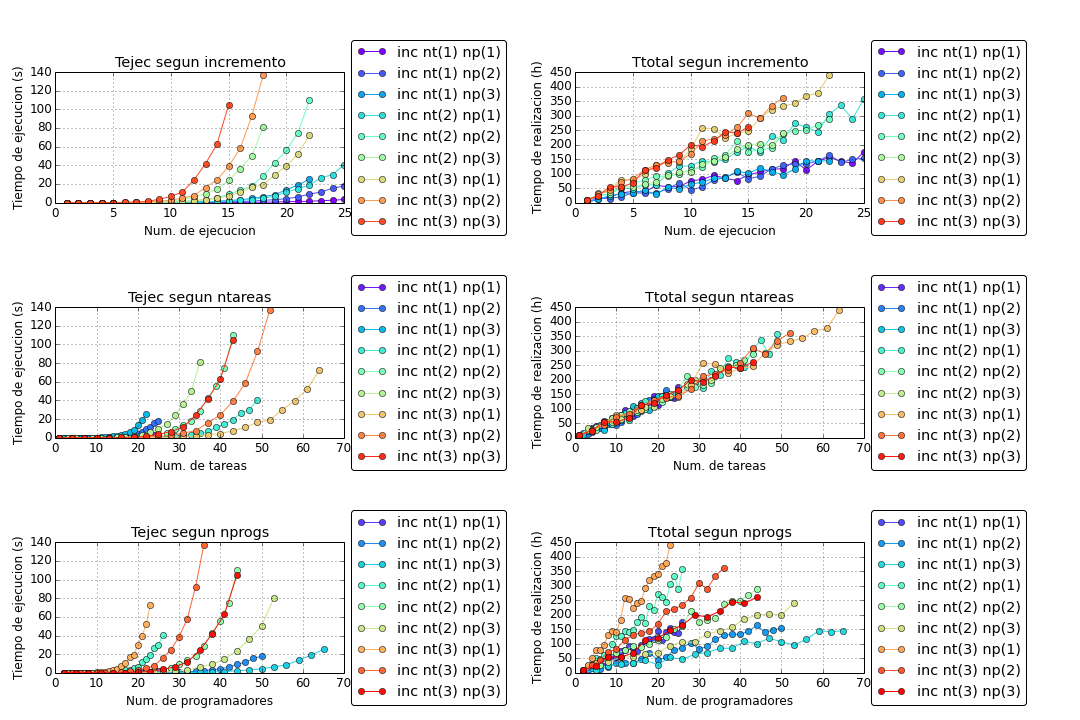
\includegraphics[height=13cm]{graph-2-1-2}
        \caption{Gráficos de los tiempos de ejecución para obtener las 
            soluciones y de los tiempos totales de desarrollo de estas en 
            función del tamaño de la entrada para la extensión 2.}
        \label{fig:extra-ext2}
    \end{figure}

\end{landscape}
}

En los gráficos de la mitad izquierda, correpondientes al tiempo de ejecución 
del \texttt{Fast Forward} para obtener la solución, se aprecia que para 
valores muy bajos la resolución es prácticamente instantánea y, a partir de 
un cierto tamaño, el tiempo de ejecución empieza a crecer de forma muy rápida 
(con los tamaños que hemos podido probar debido a las limitaciones del 
\textit{parser} del \texttt{Fast Forward} no podemos sacar conclusiones 
definitivas, pero podría tratarse de funciones polinómicas de un grado 
bastante alto, según el factor de ramificación). Esto se debe a que el 
planificador, en primera instancia, intenta encontrar una solución de forma 
rápida usando algoritmos de búsqueda local guiados por heurísticas genéricas, 
pero si no la encuentra luego procede con un algoritmo de búsqueda de tipo
\textit{best-first} que puede ser exhaustivo. Por lo tanto, para entradas 
muy pequeñas es probable que el planificador pueda hallar la respuesta con 
la primera búsqueda local pero esta ya no funcione a medida que la entrada 
crece. En este caso, como la búsqueda es prácticamente exhaustiva, el tiempo 
de ejecución depende esencialmente del factor de ramificación dado por las 
acciones del modelo.

En los gráficos de la derecha, en cambio, se representa la calidad de las 
soluciones obtenidas; es decir, la suma de las horas que los programadores 
invertirán para realizar todas las tareas asignadas en las soluciones 
obtenidas. Se aprecia claramente que, en todos los casos, este tiempo de 
resolución depende linealmente del tamaño de la entrada (básicamente del 
número de tareas). Parece muy razonable, teniendo en cuenta que los 
problemas se generan de forma aleatoria y homogénea, que el aumento del 
tiempo necesario para la realización de las tareas aumente proporcionalmente 
a la cantidad de estas (y, por lo tanto, en menor medida se aprecia en los 
gráficos una dependencia también del número de programadores, pero esto es 
porque se ha intentado mantener un cierto equilibrio entre el número de 
tareas y el número de programadores para comparar mejor la calidad de las 
soluciones). Es decir, el tiempo de resolución de las tareas depende 
linealmente del número de tareas, con una alta correlación, pero no depende 
prácticamente del número de programadores (siempre y cuando haya un número 
mínimo de programadores capaces de realizar las tareas siguiendo las 
restricciones del problema).

Se han realizado pruebas similares para todas las versiones del problema 
(las tablas y los gráficos resultantes están incluidos en los archivos 
adjuntos a este documento). El análisis de estos resultados se omite en este 
informe porque las tendencias que se aprecian en los gráficos son 
prácticamente las mismas.





\clearpage




\section{Conclusión} \label{sec:conclusion}

En este trabajo hemos resuelto un problema práctico modelizándolo como 
problema de planificación y utilizando un sistema de planificación automática
para su resolución. A pesar de tratarse de un problema relativamente simple, 
este problema nos ha permitido hacernos una idea del tipo de problemas a los 
que se pueden aplicar las técnicas de inteligencia artificial aprendidas y, 
en particular, de la capacidad expresiva de lenguajes formales como 
\texttt{PDDL} y la potencia de herramientas como \texttt{Fast Forward}.

En esta práctica, hemos analizado el problema de asignación de tareas de un 
proyecto a los programadores del equipo de desarrollo y hemos modelizado los 
elementos que intervienen en este problema mediante objetos, predicados y 
acciones de \texttt{PDDL}. Para ello, se ha seguido un desarrollo incremental 
guiado por las extensiones propuestas en el enunciado de la práctica. 

De este modo, hemos podido utilizar el planificador \texttt{Fast Forward} para 
solucionar instancias del problema debidamente seleccionadas y estudiar los 
resultados obtenidos. Así, pues, hemos podido comprobar como los sistemas de 
planificación automáticos diseñados de forma genérica y sin conocimiento del 
dominio son capaces de ofrecer buenas aproximaciones en tiempos de ejecución 
muy razonables, a pesar de su facilidad de uso y su potencia expresiva.


\clearpage



%%%%%%%%%%%%%%%%%%%%%%%%%%%%%%%%%%%%%%%%%%%%%%%%%%%%%%%%%%%%%%%%%%%%%%%%%%%%%%%%

\end{document}



